\iffalse

\chapter{Fundamentarea teoretică și documentarea bibliografică}
\label{cap:cap1}

(10–15 pagini)\footnote{Template-ul a fost construit similar celui dezvoltat de George VIERIU, disponibil la \url{https://ac.tuiasi.ro/studenti/didactic/finalizare-studii/finalizare-studii-calculatoare/finalizare-studii-calculatoare-ghidul-studentului/}}

\begin{itemize}
    \item Domeniul și contextul abordării temei;
    \item Tema propusă (formularea exactă a temei, obiective, justificarea abordării);
    \item Prezentare succintă și comparativă privind realizările actuale pe aceeași temă;
    \item Analiza tipurilor de produse/aplicații existente din respectiva categorie a temei,
tehnologii folosite pentru implementare;
    \item Elaborarea specificațiilor privind caracteristicile așteptate de la aplicație. 
\end{itemize}

Lucrările utilizate în dezvoltarea proiectului de diplomă și în redactarea tezei vor fi citate corespunzător în cadrul prezentului document. Această citare trebuie să fie o interpretare sau o descriere proprie autorului prezentei teze asupra ideii/soluției/conceptului prezentat în lucrarea sursă și \textbf{\textit{nu}} o preluare mot-a-mot sau o traducere directă. O posibilă excepție de la această regulă se poate face în cazul rezultatelor teoretice importante, cum ar fi, de exemplu, definițiile, teoremele sau algoritmii suport. În textul asociat citării este recomandat să includeți, de asemenea, și o frază prin care să realizați legătura cu lucrarea proprie. Teza capătă în acest fel consistență și evitați ideea de citare bulk, „doar ca să fie". În continuare vă prezentăm un scurt exemplu.

\todo[inline]{TO DO: Aici ar trebui să introduc o referință bibliografică deoarece ceea ce am scris nu este ideea mea}

Mironeanu et. al. propun o nouă abordare pentru monitorizarea și prevenția atacurilor cibernetice \cite{art:mironeanu:ECAD:2021}. Soluția utilizează tehnici de tip AI/ML și pe un sistem de votare ponderat cu scopul de determina dacă un acces în rețea este un acces normal sau un eventual atac. Pornind de la noțiunile descrise în \cite{art:mironeanu:ECAD:2021}, lucrarea de față își propune îmbunătățirea detecției atacurilor de tip \textit{flood}.

Pornind de la modelul REST propus de Fielding în \cite{thesis:fielding:2000} și considerând specificațiile protocolului HTTP \cite{misc:web:rfc7231}, Archip et. al. demonstrează în \cite{inproc:archip:restful:2018} faptul că o utilizare greșită a modelului amintit poate conduce la o slăbire a securității unui server. Un alt aspect important care trebuie considerat cu privire la securitatea sistemelor informatice este legat de utilizatori. Acest subiect este tratat pe larg în \cite{incollection:ARASEC2020}.

Un exemplu de intrare bibliografică pentru un \textit{tech report} este în \cite[p.~13]{IEEEexample:techreptypeii} (numărul paginii este trecut explicit în sursă). Bineînțeles, nu putem discuta despre configurările și instalările unor sisteme Cloud Computing \cite[p.~113]{book:marinescu:2018}, dacă nu considerăm și sistemele de operare suport sau gazdă \cite{book:operating_systems:2014}. În cazul în care dorim să referim o pagină web care nu se încadrează în categoriile carte, articol, raport tehnic, putem să utilizăm o intrare de tip \verb|misc| în bibliografie. Recomandarea este să utilizăm documente Web publicate de companii importante (precum IBM, RedHat, Apple, etc.) sau personalități recunoscute, precum Bruce Schneier \cite{misc:web:schneier2021}.

\textcolor{gray}{\lipsum}(Figura \ref{fig:puterea_furnizata_pe_cm_cub})

\begin{figure}[H]
    \centering
    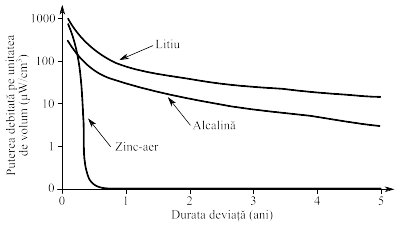
\includegraphics[width=0.6\textwidth]{continut/capitol1/figuri/puterea_furnizata_pe_cm_cub.png}
    \caption{Puterea furnizată pe cm\textsuperscript{3} relativă la durata de viață pentru trei tipuri de baterii.}
    \label{fig:puterea_furnizata_pe_cm_cub}
\end{figure}

\textcolor{gray}{\lipsum}

\section{Exemplu de subcapitol nivel 1}
\label{cap:cap1:ex-subcapitol}

\textcolor{gray}{\lipsum} (Figura \ref{fig:r2_d2})

\begin{figure}[t]
    \centering
    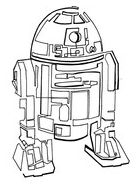
\includegraphics[width=0.25\textwidth]{continut/capitol1/figuri/r2_d2.png}
    \caption{R2-D2\protect\footnotemark}
    \label{fig:r2_d2}
\end{figure}
\footnotetext{imagine preluată de pe un site web care nu „merită” trecut la bibliografie \url{https://www.shutterstock.com/}}

\textcolor{gray}{\lipsum} 

\subsection{Exemplu de subcapitol nivel 2}
\label{cap:cap1:ex-supcapitol:nivel2}

\textcolor{gray}{\lipsum} (Figura \ref{fig:yoda})

\begin{figure}[H]
    \centering
    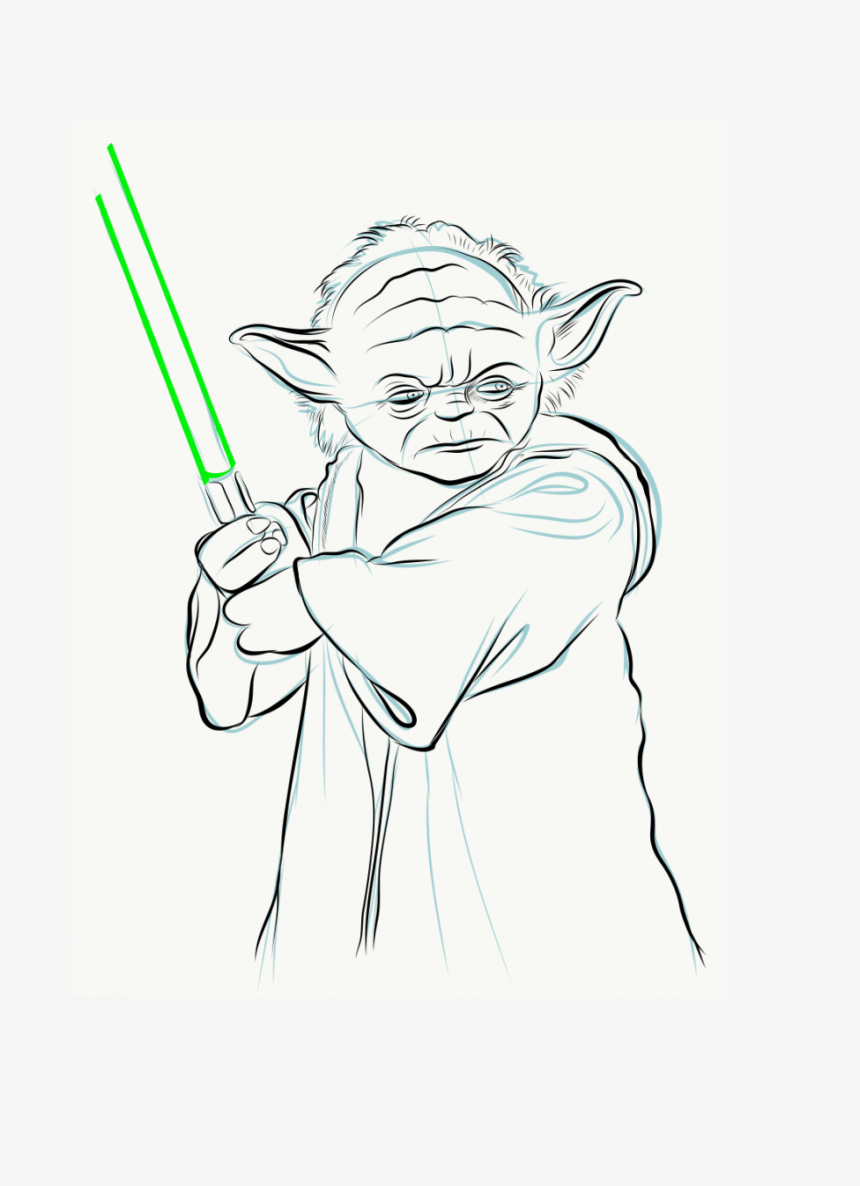
\includegraphics[width=0.3\textwidth]{continut/capitol1/figuri/yoda.png}
    \caption{Yoda\protect\footnotemark}
    \label{fig:yoda}
\end{figure}
\footnotetext{imagine preluată de pe un site web care nu „merită” trecut la bibliografie \url{https://www.pngitem.com/}}

\textcolor{gray}{\lipsum}

\subsubsection{Exemplu de subcapitol nivel 3}
\label{cap:cap1:ex-subcapitol:nivel2:nivel3}

\textcolor{gray}{\lipsum}

Următoarele e fără label FTW, decât să demonstrez gen!\footnote{Dacă vă prindem cu astfel de exprimări, vă scădem 2 puncte!!!}

\section{Nivel 1}
\label{cap:cap1:nivel1}

\subsection{Nivel 2}
\label{cap:cap1:nivel1:nivel2}

Ghilimelele se pun înainte și după reproducerea unui text. Se pun între semnele citării cuvintele sau grupurile de cuvinte citate ironic sau care redau atitudinea rezervată ori dezaprobatoare a autorului față de realitățile pe care le desemnează respectivele cuvinte. Se obișnuiește să se pună între ghilimele titlurile operelor literare de artă sau științifice, ale publicațiilor, numele instituțiilor, firmelor etc. atunci când aceste titluri sunt reproduse într-o frază. 
Atenție: Ghilimelele limbii engleze (“ ”) sunt diferite de ghilimelele limbii române („ ”)!
Observație: Documentele tehnice au adoptat din sintaxa limbajelor de programare ghilimelele duble (") pentru a evidenția șirurile de caractere în text și ghilimelele simple (') pentru evidențierea caracterelor. De exemplu: "acesta este un șir de caractere", acesta este caracterul 'x'.

\subsubsection{Nivel 3}
\label{cap:cap1:nivel1:nivel2:nivel3}

Oricum, mai departe de \verb|#.#.#.#| \textbf{\textit{NU}} trebuie să se ajungă :P.

\fi


\chapter{Fundamentarea teoretică și documentarea bibliografică}
\label{cap:cap1}

Structura următoarelor câteva subcapitole este puternic influențată de structura cursului de Calcul Cuantic din cadrul Facultății de Informatică de la Universitatea "Alexandru Ioan Cuza" \cite{misc:web:QCCuza}, predat de doamna Conf. Arusoaie Andreea , fără de care această lucrare probabil că nu ar fi fost posibilă.